\documentclass[conference]{IEEEtran}
\IEEEoverridecommandlockouts
% The preceding line is only needed to identify funding in the first footnote. If that is unneeded, please comment it out.
\usepackage{cite}
\usepackage{amsmath,amssymb,amsfonts}
\usepackage{graphicx}
\usepackage{textcomp}
\usepackage{enumitem}
\usepackage{xcolor}
\usepackage{times}
\usepackage[binary-units=true]{siunitx}
\usepackage{latexsym}
\usepackage{hyperref}
\hypersetup{colorlinks=true,linkcolor=black,citecolor=blue,filecolor=black,urlcolor=blue}
\usepackage{algpseudocode}
\usepackage{algorithm}
\usepackage{caption}
\usepackage{subcaption}

%\setlength{\textfloatsep}{7pt}

\newcommand{\TG}[1]{\color{cyan}From Tristan: #1 \color{black}}
\newcommand{\MD}[1]{\color{magenta}From Mathieu: #1 \color{black}}
\newcommand{\VHS}[1]{\color{green}From Valerie: #1 \color{black}}

\begin{document}

\title{Performance comparison of Dask and Apache Spark on HPC systems}

\author{Mathieu Dugr\'e, Val\'erie Hayot-Sasson, Tristan Glatard\\
	Department of Computer Science and Software Engineering\\
	Concordia University, Montr\'eal, Qu\'ebec, Canada\\
	\{mathieu.dugre, valerie.hayot-sasson, tristan.glatard\}@concordia.ca
	\vspace*{0.8cm} % to avoid weird spacing of 1st page by Latex.
}

\maketitle

\begin{abstract}
	% TODO
\end{abstract}

\begin{IEEEkeywords}
	Performance, Big Data, Dask, Spark, Neuroimaging, HPC
\end{IEEEkeywords}

\section{Introduction}
The rise in data sharing coupled with improved data collection technologies lead neuroimaging into the Big Data era\cite{ALFAROALMAGRO:18, van2014human}. \MD{cite CONP portal}
While common neuroimaging workflow engines, such as Nipype\cite{Nipype:11}, are well rounded to process standard compute-intensive pipeline,
they lack Big Data strategies (i.e. in-memory computing, data locality, and lazy-evaluation) to improve the performance of increasingly prevalent data-intensive pipelines.
A previous study\cite{hayot2019performance} noted the importantce of in-memory computing and data locality to improve the performance of data-intensive pipelines.
In this work, we study how performance benchmarks generalize accross Big Data engines in an HPC environement.
In particular, we study the detailed performance difference between Dask\cite{Dask:15} and Apache Spark\cite{Spark:16}, for their suitability to process neuroimaging pipelines.
Our objective is to assess whether Spark or Dask has substantial performance benefits to process data-intensive pipeline in HPC clusters.

Spark and Dask both provide in-memory computing, data locality, and lazy-evaluation, which is common for Big Data engines.
Both of their scheduler operate dynamically, which benefit applications with runtime unknown ahead of time\cite{Dask:15}.
They also provide rich high-level API and support a variety of schedulers and deployment environment, such as Mesos\cite{hindman2011mesos}, YARN\cite{vavilapalli2013apache}, Kubernetes, and HPC clusters.
Although sharing similarities, these engines have differences.

First and foremost, Spark is written in Scala while Dask is in Python.
Given the popularity of Python in the scientific community, this arguably gives a edge to Dask due to the serialization cost between Python and Scala.
However, if not careful, the Python Global Intepreter Lock (GIL) can significatly reduce the parallelism of an application, in some cases.
The difference in programmming language also provides different benefits.
On the one hand, as part of the Scipy ecosystem, Dask provides almost transparent integration with APIs such as Numpy arrays, Pandas dataframe, or RAPIDS GPU accelerated code framework.
On the other hand, Spark's Java, Scala, R, and Python APIs allow to easily parallelize pipelines with minimal performance loss, thanks to the Java Virtual Machine \TG{you could add a few words to explain why the JVM is useful for parallelization ("thanks to the JVM that ...")}.
Our study is restrained to performance, although, we recognize that other factors affect the choice of an engine in practice.

While laptops or workstations can be sufficient for some applications, data-intensive neuroimaging pipelines often require large infrastructures.
This paper focuses on the performance of Big Data engines in HPCs environments.
We installed the Slurm scheduler and Lustre file system~\cite{braam2019lustre} on a dedicated cluster to mimic a typical HPC system.
Lustre is a powerful and scalable file system for HPC environement offering parallel file accesses.

In a previous study\cite{8943502} we found that their was no significant performance difference between Apache Spark and Dask for data-intensive application.
However, due to the use of the network file-system (NFS) the performance of the applications was limited by an I/O bottleneck.
Another study \cite{8588652} also reported network and I/O bottlenecks when concurrency increased.
This same study found that the startup overhead time for Spark was larger than for Dask.
On the contrary, the work in~\cite{Mehta:17} claims that the startup overhead is larger for Dask than for Spark.
This suggests that the startup overhead might vary depending on cluster configuration.
The latter study processed a \SI{100}{\giga\byte} dataset using a neuroimaging pipeline and found Dask to be up to 14\% faster than Spark due to ``more efficient pipelining" and serialization time to Python.
On the contrary, the work in \cite{10.1145/3225058.3225128} shows that with large datasets, Spark provides better speedup than Dask.
However, that study used the Dask Bag API which is know to have performance limitation compared to other Dask APIs.
The above studies compared the engines performance at a high-level.
In comparison, our study provides a detailed analysis of the performance differences and similarities between Dask and Spark for data-intensive applications.


The next section introduce the Lustre file system and the Big Data engines.
Next, we present the design of our benchmarking experiments.
We consider two types of data-intensive neuroimaging pipelines: high-resolution imaging and large functional MRI studies.
The pipelines we chose involve different compute and I/O patterns; e.g. map-reduce or map-only and requiring partial data in memory or the whole dataset.
Further sections present our results, discussion, and conclusion.


\section{Background}
\subsection{Lustre}
The Lustre file-system is a parallel file system well suited for HPC environments.
Lustre offers a POSIX compliant interface with the file system.
Installed in some of the most powerful supercomputer, Lustre is designed to scale to thousands of nodes, petabytes of storage, and hundreds of gigabits per second of I/O throughput.

At the core of Lustre are the \textit{management servers} (MGSs) and \textit{metatdata server} (MDSs) in charge of the files operations and metadata,
the \textit{object storage targets} (OSTs) to store file data, and the \textit{obejct sotrage server} (OSSs) to handle the OSTs.
Lustre clients make requests to the MGSs to access files on the OSTs.
To handle failures in the system, the MGSs, MDSs, and OSTs have failover capabilities.
InfiniBand, Ethernet, or a combination of both can be used to interconnect these different components.

\subsection{Dask}
Dask is a Python-based Big Data engine with growing popularity in the scientific Python ecosystem.
Dask was designed with data locality and in-memory computing in mind, to mitigate the data transfer bottleneck in Big Data workflows.
Data locality, popularized by Map-Reduce \cite{dean2008mapreduce}, schedules tasks where the data reside.
In-memory computing minimizes the overhead of transferring data to disk by keeping data in memory when possible.
Dask uses lazy evaluation to reduce unnecessary communication and computation.
The engine builds a dynamic graph before execution, allowing it to determine which task to compute.
Dask workflows can further reduce data transfer by leveraging multithreading whenever the Python GIL does not restrict it.
Fault-tolerance is achieved by recording data lineage, the sequence of operations used to modify the initial data.

Dask offers five data structures:
\href{https://docs.dask.org/en/latest/array.html}{Array},
\href{https://docs.dask.org/en/latest/bag.html}{Bag},
\href{https://docs.dask.org/en/latest/dataframe.html}{DataFrame},
\href{https://docs.dask.org/en/latest/delayed.html}{Delayed},
and \href{https://docs.dask.org/en/latest/futures.html}{Futures}.
Arrays offer a clone of NumPy API for distributed processing of large arrays.
Bags are a distributed collection of Python object that offers a programming abstraction similar to \href{https://toolz.readthedocs.io/en/latest/}{PyToolz}.
Dataframes are a parallel composition of \href{https://pandas.pydata.org/}{Pandas} Dataframes used to process a large amount of tabular data.
Dask Delayed offers an API for distributing arbitrary functions that do not fit in the above frameworks.
Lastly, Dask Futures can also execute arbitrary functions; however, it launches computation immediately rather than lazily.
Dask allows users to install only required components making it lightweight.

In Dask, a scheduler decides where and when to execute tasks using the Dask graph.
API operations generate multiple fine-coarse tasks in the computation graph, allowing a more straightforward representation of complex algorithms.

The Dask engine is compatible with multiple distributed schedulers, including YARN and Mesos.
Dask also provides its own \textit{Dask Distributed scheduler}.
We chose to use Dask Distributed scheduler to keep the environment balanced between the engines.

In the Dask Distributed scheduler, a \textit{dask-scheduler} process administrates the resource provided by  \textit{dask-worker}s in the cluster.
The scheduler receives jobs from clients and assigns tasks to available workers using a LIFO (Last-In-First-Out) job scheduling policy.
That is an utter process branch of the Dask graph before proceeding with the next one \TG{No comprendo, please revise syntax :)}.

Dask offers multiple ways to deploy a cluster, including, but not limited to, SSH configs, Kubernetes, SLURM, PBS.
For our experiments, we used the \href{https://jobqueue.dask.org/en/latest/generated/dask_jobqueue.SLURMCluster.html}{Dask SLURM cluster} API.

\subsection{Apache Spark}
Apache Spark is a widely-used general-purpose Big Data engine.
Like Dask, it aims at reducing data transfer costs by incorporating data locality, in-memory computing, and lazy evaluation.

Spark offers three options to schedule jobs: Spark Standalone, Mesos, and YARN.
Spark Standalone is a simple built-in scheduler.
YARN is mainly used to schedule Hadoop-based workflows, while Mesos can be used for various workflows.
We limit our focus to Spark Standalone scheduler, as researchers are likely to execute their workflows in an HPC environment where, usually, neither YARN nor Mesos is available.

In the Spark Standalone scheduler, a \textit{leader} (a.k.a master) coordinates the resource provisioned by \textit{workers} in the cluster.
A \textit{driver}  process receives jobs from clients and requests workers from the leader.
Jobs are divided into stages to be executed onto workers.
Each operation in a stage is represented by a high-level task in the computation graph.
Like Dask, Spark Standalone scheduler uses a LIFO policy to schedule tasks.
Spark Standalone has two execution modes: (1) the client mode, where the driver process runs in a dedicated process,
and (2) the cluster mode, where the driver runs within a worker process.
Our experiments use the client mode since cluster mode is not available in PySpark.

Spark's primary data structure is Resilient Distributed Dataset (RDD)\cite{RDD}, a fault-tolerant, parallel collection of data elements.
RDDs are the basis of the other Spark data structure: Datasets and DataFrames.
Datasets are similar to RDD but benefit additional performance by leveraging the Spark SQL's optimized execution engine. 
The DataFrames are Datasets organized into named-columns and are used to process tabular data. 
While the DataFrame API is available in all supported languages, Datasets are limited to Scala and Java. 

Python is a standard programming language in the scientific community, offering numerous data processing libraries.
While serialization from Python to Java, an operation required when using Spark's Python API, creates overhead, we found it minimal \cite{8943502}.
We focus on PySpark API to have a more balanced environment between the different engines and for its suitability to neuroimaging.

\section{Methods}
\subsection{Infrastructure}
We used the ``slashbin" cluster at Concordia University.
The cluster has 8 compute nodes, 4 storage nodes, 1 login node, and 1
Lustre metadata node. Each
compute node has 2 $\times$ 16-core Intel(R) Xeon(R) Gold 6130 CPU
@ 2.10GHz, 256~GiB of RAM, 6 $\times$ SSDs of 450~GiB each with the XFS
file system (no RAID enabled), 378~GiB of tmpfs, 126~GiB of devtmpfs file system,
CentOS~8.1 and Linux kernel
\textit{4.18.0-240.1.1.el8\_lustre.x86\_64}.

\TG{describe the Lustre installation: data nodes and lustre config}
\TG{Use GB or GiB consistently}

Both Spark and Dask were configured to have 8 worker processes each with 8
threads. Each worker was allocated \SI{31.5}{\giga\byte} of memory \TG{,
	determined as the amount of memory that ...}. \TG{any other Spark or Dask
param? Location of log files, etc} A new Dask or Spark cluster was started and
teared down for each experiment.

Dask ?? and Spark ?? \MD{Add version when after locking it for experiments.} was used for our experiments.

\subsection{Dataset}
We used BigBrain\cite{Amunts:13}, a 3-D image of the human brain with voxel
intensities ranging from 0 to 65,535. We converted the blocks into the
NIfTI format, a popular format in neuroimaging. We left the NIfTI blocks
uncompressed, resulting in a total data size of \SI{648}{\giga\byte}. To
evaluate the effect of block size, we split the image into 1000, 2500,
and 5000 files of \SI{648}{\mega\byte}, \SI{259.2}{\mega\byte}, and
\SI{129.6}{\mega\byte}, respectively. The
\href{https://github.com/big-data-lab-team/sam}{sam} library was used to
split the image.

We also used the dataset provided by the Consortium for Reliability and
Reproducibility
(\href{http://fcon_1000.projects.nitrc.org/indi/CoRR/html/}{CoRR})
\cite{zuo2014open}, freely available on
\href{https://datasets.datalad.org/?dir=/corr/RawDataBIDS}{DataLad}. The
entire dataset is \SI{408.4}{\giga\byte}, containing anatomical, diffusion
and functional images of 1,397 subjects acquired in 29 sites. We used all
3,491 anatomical images, representing \SI{39}{\giga\byte} overall
(\SI{11.17}{\mega\byte} per image on average).

\subsection{Applications}
In this section, we describe the applications used to benchmark Dask and Spark.
We use three simple synthetic applications to have a deep understanding of the 
underlying behavior of the applications with simple I/O pattern; namely
\textit{Increment}, \textit{Multi-Increment}, and \textit{Histogram}.
Also, two neuroimaging applications are used to study more realistic 
applications; namely \textit{Kmeans} and \textit{BIDS App Example}.

To have a fair comparison between the engines, the code base for the core functions of the applications is the same for both engines.
This allow us to reduce the performance difference from different implementations.
Note that this is not the case for the \textit{Kmeans} application as the best performing API for Dask and Spark differed largely in term of implementation.

\subsubsection{Increment}
We adapted the increment application used in \cite{hayot2019performance}.
This synthetic application reads blocks of the BigBrain from Lustre and
simulates computation by sleeping for a specified period. To simulate
intermediate results, we repeat the sleep process for a configurable amount
of time. We prevent data caching of the blocks by incrementing their voxels
value by one after each sleep operation. Finally, we write the resulting
NIfTI image back to Lustre. This application allows us to study the engines
when their inputs are processed independently. The map-only pattern
mimics the processing of multiple independent subjects in parallel.


\begin{figure}[!ht]
	\centering
	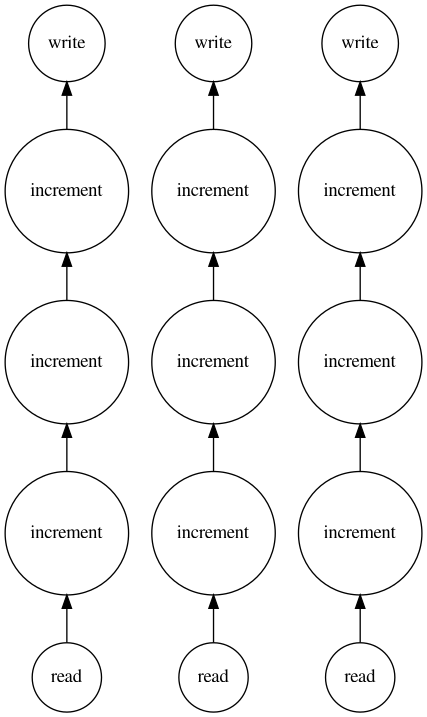
\includegraphics[height=\columnwidth,
	angle=0]{figures/increment.png}
	\caption{Task graph for Incrementation with 3 iterations and 3 BigBrain blocks.}
	\label{fig:graph-increment}
\end{figure}

% Currently ommitted due to issue with memory.
% 
% \subsubsection{Multi-Increment}
% Our second application is an adaptation of the increment application. A
% significant difference is that, at each iteration, it uses a random
% BigBrain block as the increment value. This change allows the
% multi-increment application to have inter-worker communication while
% remaining simple.

% \begin{figure}[!hb]
% 	\centering
% 	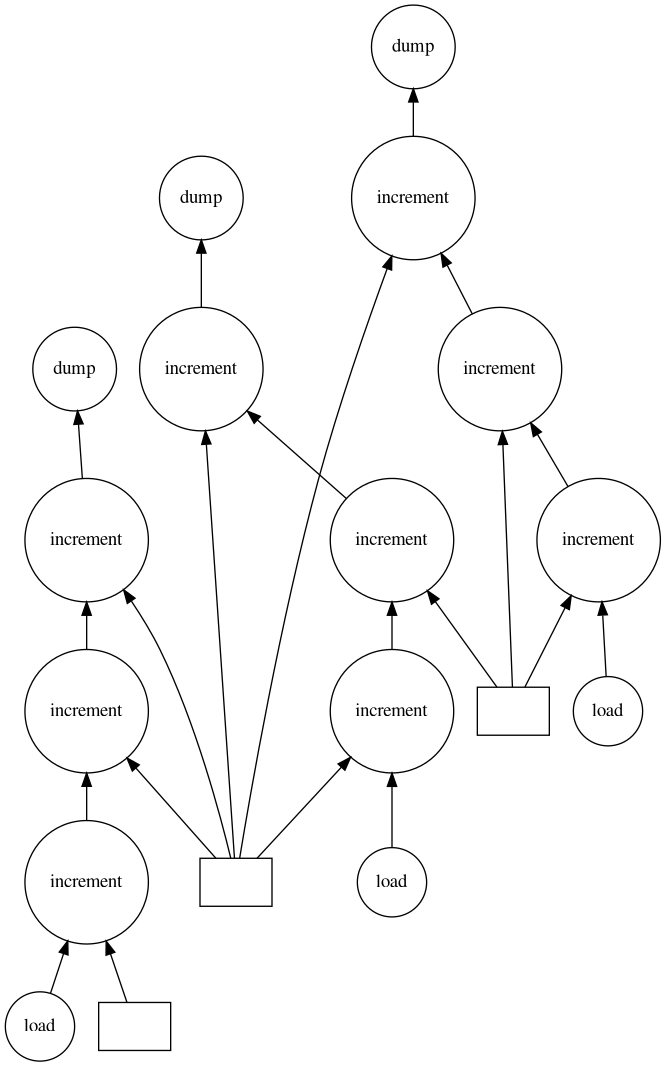
\includegraphics[height=\columnwidth,
% 	angle=0]{figures/multi-increment.png}
% 	\caption{Task graph for Multi-Incrementation with 3 iterations and 3 BigBrain blocks.}
% 	\label{fig:graph-muti-increment}
% \end{figure}
	
\subsubsection{Histogram}
As our third application, we calculate the histogram of the BigBrain image. 
The application reads the BigBrain blocks from Lustre, calculates each intensity's frequency, and then writes the aggregated result back on Lustre.
This map-reduce application has a very high read overwrite ratio.
Moreover, this application requires shuffling, albeit of a limited amount of data. 
The amount of inter-worker communication is in-between the increment and multi-increment applications.

\begin{figure}[!hb]
	\centering
	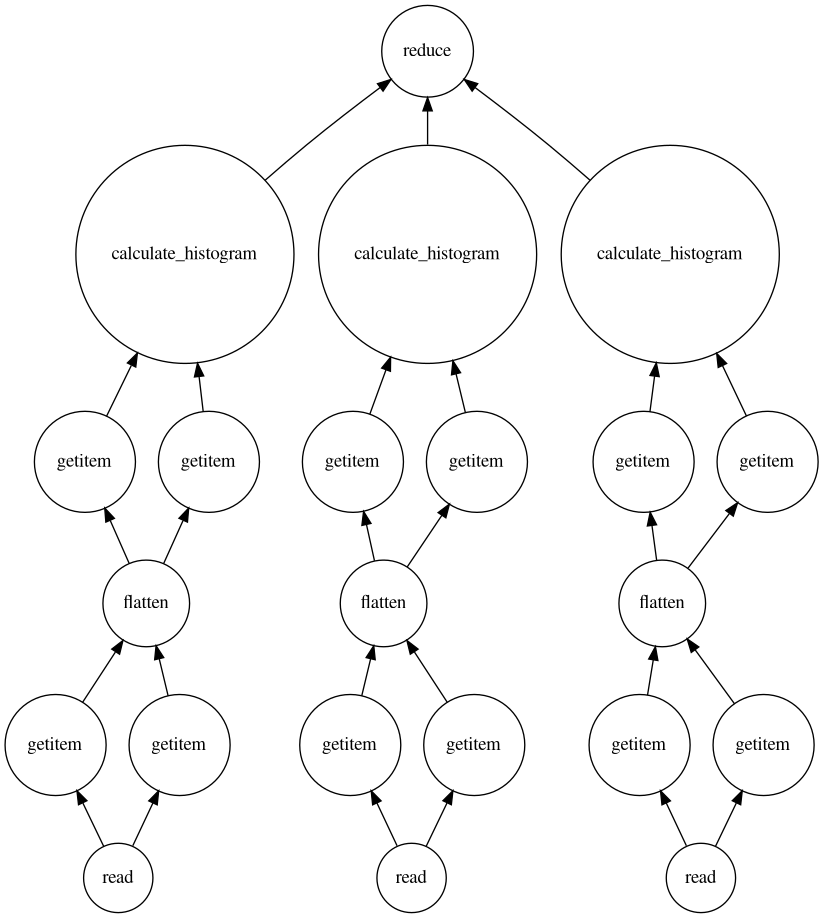
\includegraphics[height=\columnwidth,
	angle=0]{figures/histogram.png}
	\caption{Task graph for Histogram with 3 BigBrain blocks.}
	\label{fig:graph-histogram}
\end{figure}
	
\subsubsection{Kmeans}
For our fourth application, we apply Kmeans clustering to the voxel
intensities of the BigBrain image. We set the number of clusters to 3. The
application starts by reading the image blocks, combining all voxels in a
1-D array, and choosing initial centroids using the min, max, and
intermediate values. It assigns each voxel to its closest centroid and
updates each centroid with the average of its assigned voxels. It repeats
the assignment and update steps for a configurable number of iterations.
Finally, the voxels of the image blocks are classified and written back to
the file system. Updating the centroids involves substantial data
communication between the workers.

For this application, the Spark and Dask implementations differ slightly,
to take advantage of the best-suited API from both engines. The Spark
implementation uses the Map-Reduce paradigm, while the Dask one uses array
programming.
	
	
\subsubsection{BIDS App example}
Our fifth application is BIDS App example, a neuroimaging pipeline to
measure the brain volume from MRIs. For this application, we use the CoRR
dataset. The application extracts the brain volume of each participant,
then computes the average for each group of participants. Unlike the other
applications, BIDS App example is a command-line executed in a Docker image
(bids/example on DockerHub). We converted the Docker image to a Singularity
image for use in HPC environments, \MD{Cite paper on reason why this is
done.} using
\href{https://hub.docker.com/r/singularityware/docker2singularity/tags/}{docker2singularity}

\TG{You should explain how the applications were implemented in Dask and
Spark which APIs were used and why, etc}

\subsection{Experiments}
Table~\ref{table:parameters} shows the parameters that were varied
throughout the experiments. We varied (1) the number of workers to assess
the scalibility of the engine scheduler, (2) the BigBrain
block size in Increment, Multi-Increment, and Histogram to measure the
effect of different I/O patterns and parallelization degrees, (3) the
number of iterations to evaluate the effect of number of task, and (4) the
sleep delay to study the effect of task duration. It should note that
increasing the number of iterations for a given sleep delay also increases
the total compute time of an application.

To avoid potential external biases due to caching, background processes and
network load, we ran the applications in randomized order and cleared the
page cache in between every experiments. Each benchmark was run ten times.

For each run, we measured the makespan of the application as well as the
cumulative time spent in the different functions for read, processing, and
writing data. The overhead calculation for each CPU thread is the end time
of the last processed task minus the total runtime of the tasks ran for
this thread \TG{unclear definition. Don't refer to CPU threads as a given task may be executed on more than 1. Maybe refer to engine executors?}. Summing those results gives the total overhead for the
application.

%  TODO Fix table for the final parameters/applications used.
\begin{table*}[t]
	\renewcommand{\arraystretch}{1.5}
	\caption{Parameters for the experiments}\label{table:parameters}
	\centering
	\begin{tabular}{|l|c|c|c|c|c|}
		\hline & Increment & Multi-Increment & Kmeans & Histogram & BIDS App Example \\\hline
		\# of Nodes & \multicolumn{5}{c|}{2, 4, 8} \\\hline
		Dataset size [\SI{}{\giga\byte}] & 648 &\multicolumn{2}{c|}{486} & 648 & \multicolumn{1}{c|}{39} \\\hline
		Number of file & \multicolumn{4}{c|}{1000, 2500, 5000}  & \multicolumn{1}{c|}{3491} \\\hline
		\# of Iterations & 1, 5, 25 & \multicolumn{2}{c|}{1, 3, 9}                 & \multicolumn{2}{c|}{-} \\\hline
	\end{tabular}
\end{table*}

\section{Results}
\subsection{Increment}
Figure \ref{fig:increment_worker} depicts the total execution time spent in each code segment of the \textit{Increment} application.
The bars are broken down into Idle, Read, Write, and other application specific functions.
The mean of each bar was calulated from 10 repetitions, with the error bar representing the standard deviation.
As expected, the compute time, from \textit{Increment}, remains the same when we vary the number of nodes.
However, the \textit{Load} and \textit{Dump} time increase with the number of nodes for both engines.
This is explained by an I/O bottleneck on the Lustre file system.

From Figure \ref{fig:increment_worker}, we also observe that Dask's overhead is higher than Spark's.
While the overhead of both engines increases with the number of nodes, Dask's overhead is significantly worse when scaling.
Althought Dask has higher overhead, the total time for both engine is similar; with a maximum makespan difference of \SI{7}{\second} for 2 nodes.
This is due to a tradeoff between disk bandwidth and compute/idle time.
When a multiple threads access Lustre concurrently, they shared the disk bandwitdth resulting in longer I/O time.
However, when most threads are either idle or performing computations, it reduce the contention on the disk bandwitdh.
\begin{figure}[!h]
	\centering
	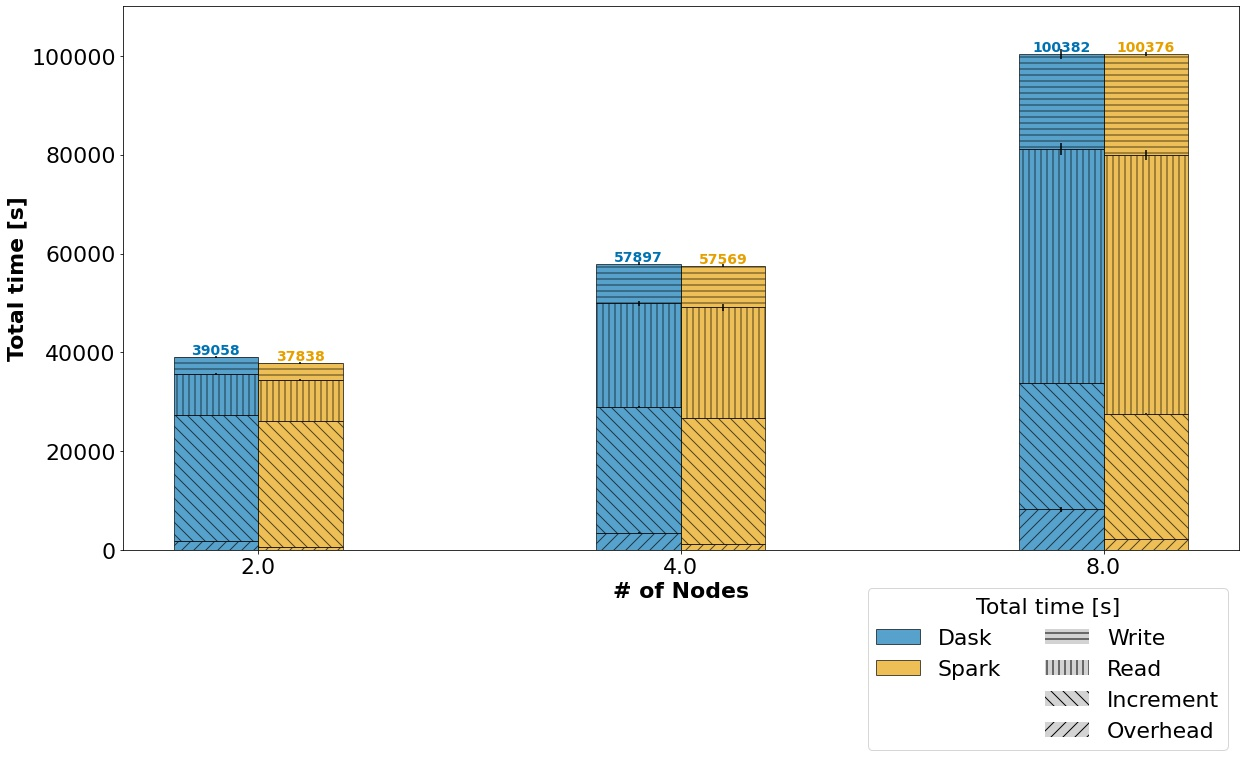
\includegraphics[clip,width=\columnwidth]{figures/stacked_increment_worker.jpg}
	\caption{Increment: varying nodes -- 5000 files, 5 iterations, \SI{1}{\second} delay}
	\label{fig:increment_worker}
\end{figure}

Figure \ref{fig:increment_itr} shows the detailed execution time for the \textit{Increment} application while varying the number of iterations.
As expected, the idle time for both engines increases with the number of iterations.
However, idle time for Dask increase significantly faster that Spark; resulting in a \SI{38}{\second} makespan difference for 25 iterations.

Figure \ref{fig:increment_itr} also depicts that as the total computation time increases the total I/O time decreases.
This is explained by an I/O bottleneck on the Lustre file system.
When threads are busy with computations they reduce the contention on Lustre, thus improving I/O speed for individual accesses.
%  # of iterations
\begin{figure}[!h]
	\centering
	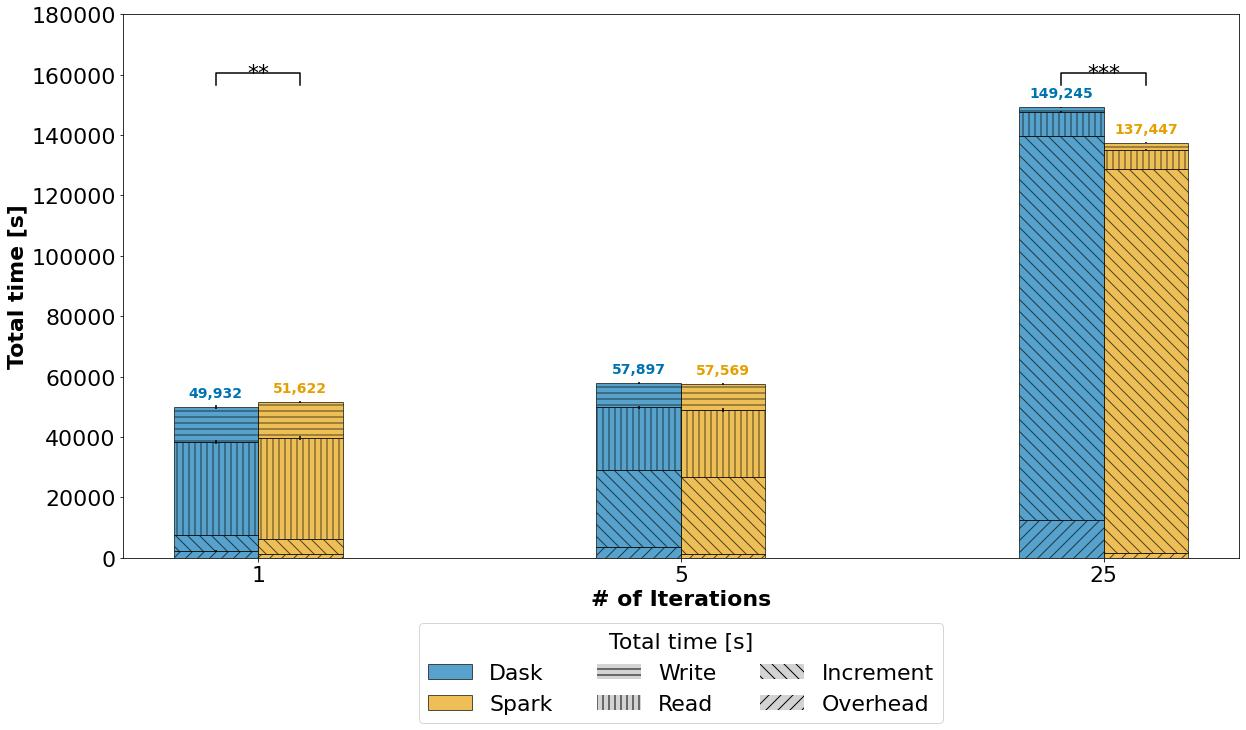
\includegraphics[clip,width=\columnwidth]{figures/stacked_increment_itr.jpg}
	\caption{Increment: varying iterations -- 4 nodes, 5000 files, \SI{1}{\second} delay}
	\label{fig:increment_itr}
\end{figure}

Figure \ref{fig:increment_block} shows an increase in \textit{Increment} time.
This is because the increment is performed on each file.
Thus increasing the number of file increase the computation time.
Similarly to Fig. \ref{fig:increment_itr} increasing the total compute time of the application reduce the total I/O time.
Again, this is explain by the I/O tradeoff between compute time and contention of disk bandwidth.

From figure \ref{fig:increment_block} we also observe that Dask has significantly higher idle time than Spark.
However, the total of the application is similar due to the tradeoff between I/O and compute/idle time.

% # of files
\begin{figure}[!h]
	\centering
	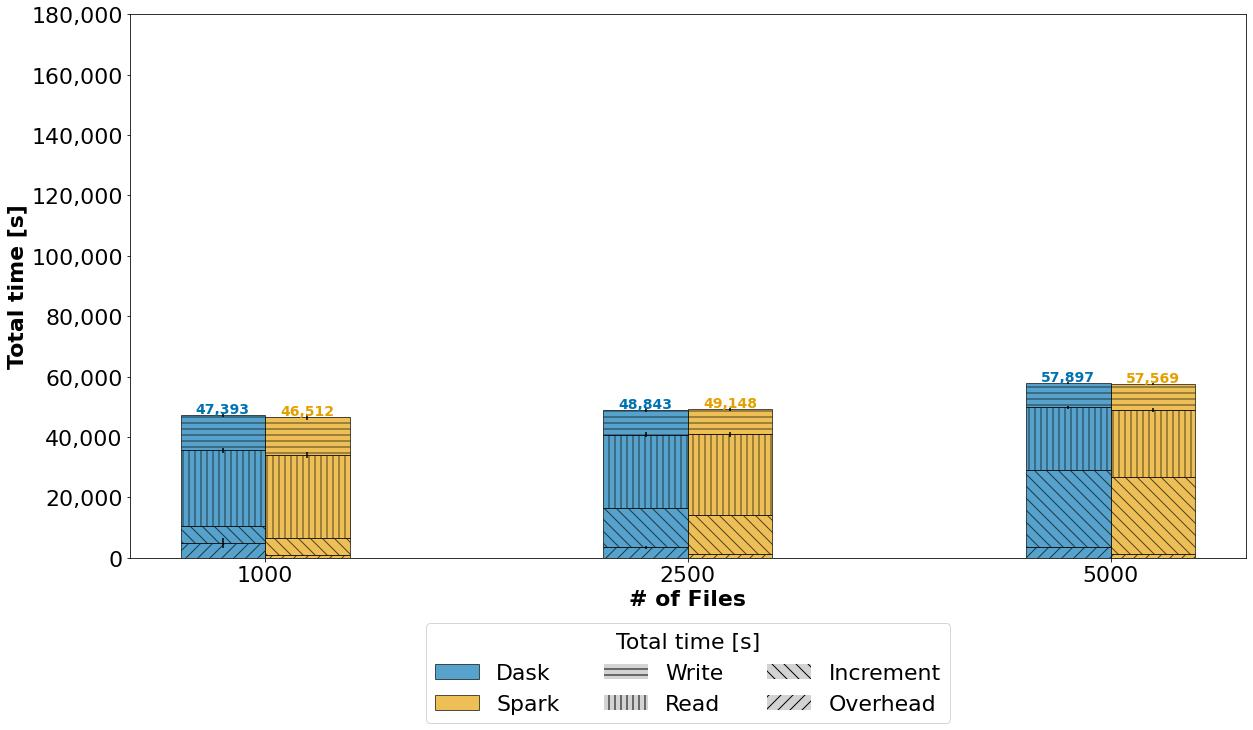
\includegraphics[clip,width=\columnwidth]{figures/stacked_increment_block.jpg}
	\caption{Increment: varying \# of files -- 4 nodes, 5 iterations, \SI{1}{\second} delay}
	\label{fig:increment_block}
\end{figure}



% \subsection{Multi-Increment}
% TODO: experiment
% Memory issue with Spark (Heap space runs out of memory)

\subsection{Kmeans}


\subsection{Histogram}
Figure \ref{fig:histogram_worker} depicts the execution time for the \textit{Histogram} when varying the number of nodes.
Overall, Spark has upt to 5\% lower total execution time with the difference comming from a shorter execution time for \textit{Calculate\_histogram}.
This is unexpected as the code base for both engine is the same; with only the calling APIs differing.
% This happened for both Bags and Delayed. There might be a higher serialization cost.
As with previous experiments, the overhead for Spark is less and scale better, although, compensated by a longer total I/O time.
% # of nodes
\begin{figure}[!h]
	\centering
	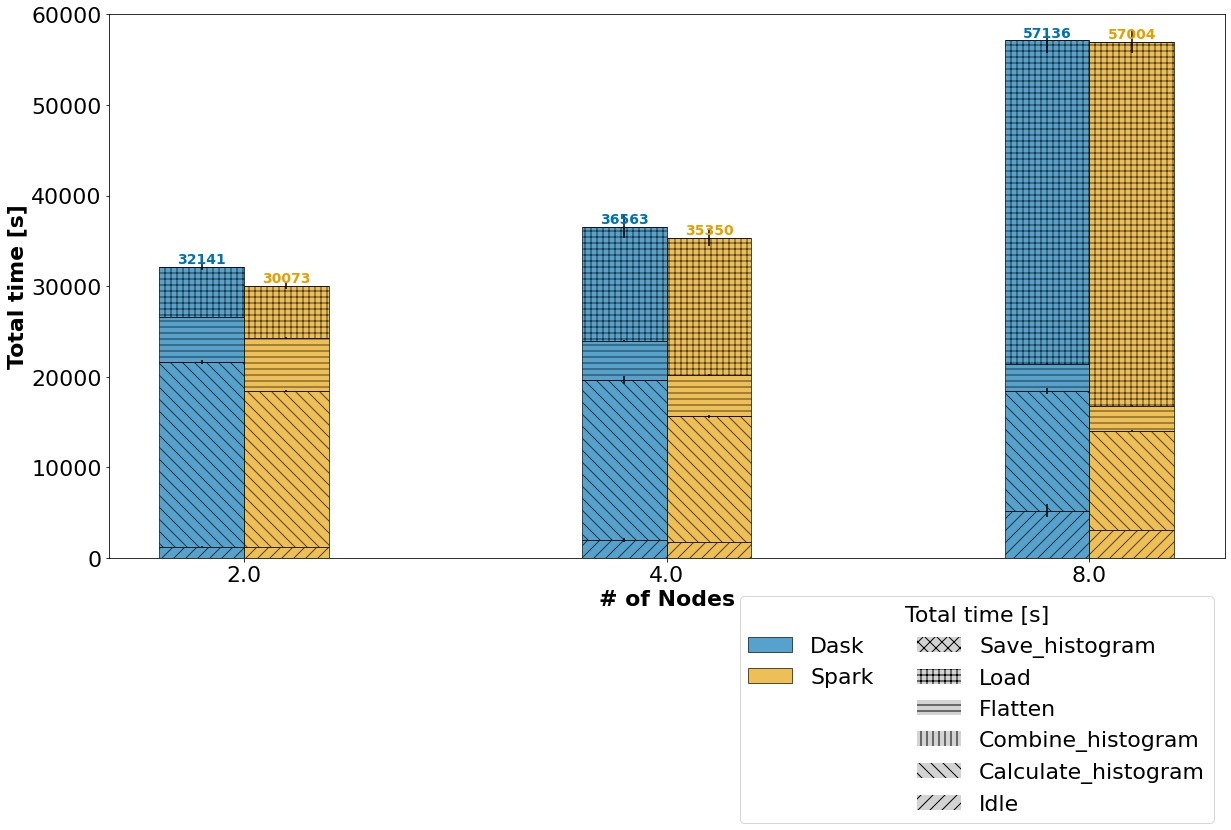
\includegraphics[clip,width=\columnwidth]{figures/stacked_histogram_worker.jpg}
	\caption{Histogram: varying nodes -- 5000 files, 5 iterations, \SI{1}{\second} delay}
	\label{fig:histogram_worker}
\end{figure}

Figure \ref{fig:histogram_worker} shows the execution time for the \textit{Histogram} when varying the number of files.
The results are similar to varying the number of nodes with Spark having faster compute time for \textit{Calculate\_histogram}.
However, the makespan difference is much smaller due to larger I/O time for both engine.
%  # of files
\begin{figure}[!h]
	\centering
	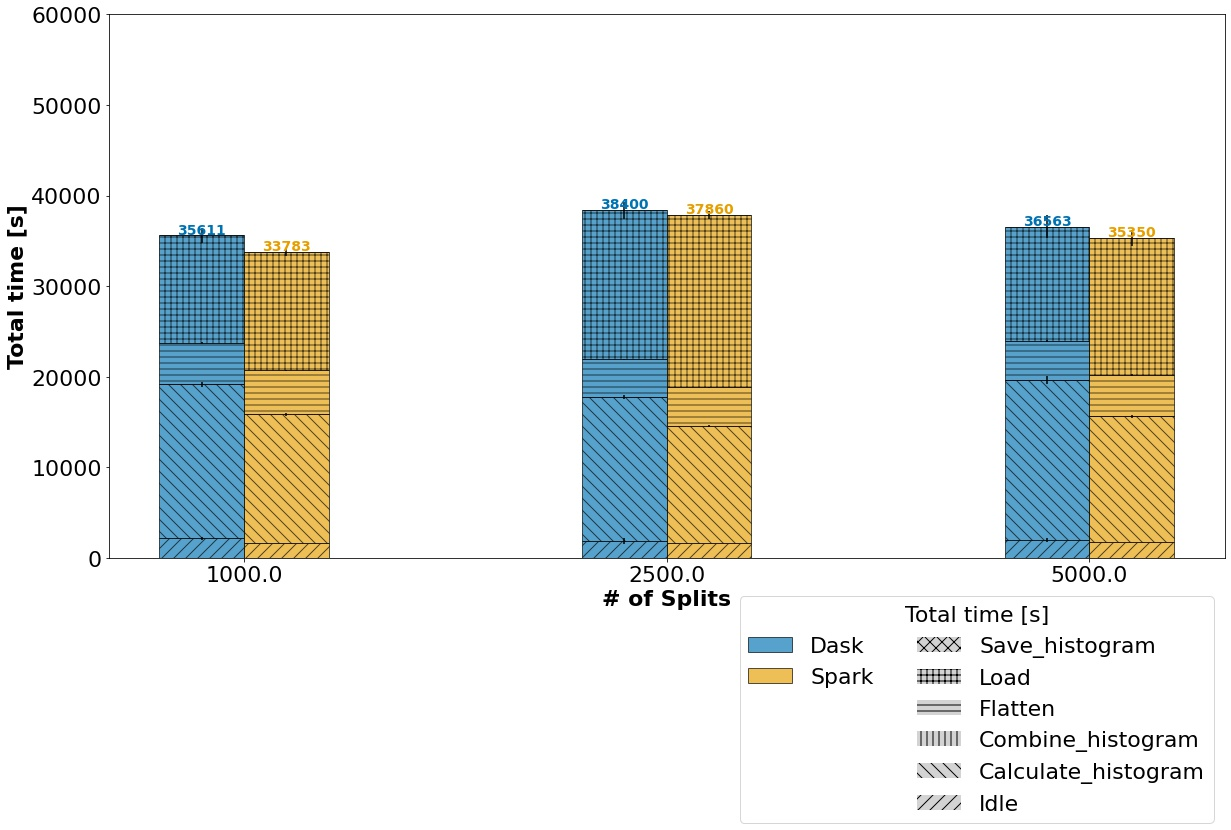
\includegraphics[clip,width=\columnwidth]{figures/stacked_histogram_block.jpg}
	\caption{Histogram: varying \# of files -- 4 nodes, 5 iterations, \SI{1}{\second} delay}
	\label{fig:histogram_block}
\end{figure}

\subsection{BIDS App Example}
Figure \ref{fig:bids} shows the total execution time for the \textit{BIDS App example} application when varying the number of nodes.
We observe that Dask has significantly lower execution time than Spark; between 10\% to 15\%.
The main difference comes from a increased amount of stagger tasks for Spark, thus increasing the idle time of the application.
Moreover, a shorther cluster deployement time for Dask reinforce the difference in idle time.
As with other experiments, the I/O from Lustre affects the scaling of both engines as we increase the number of nodes.
\begin{figure}[!h]
	\centering
	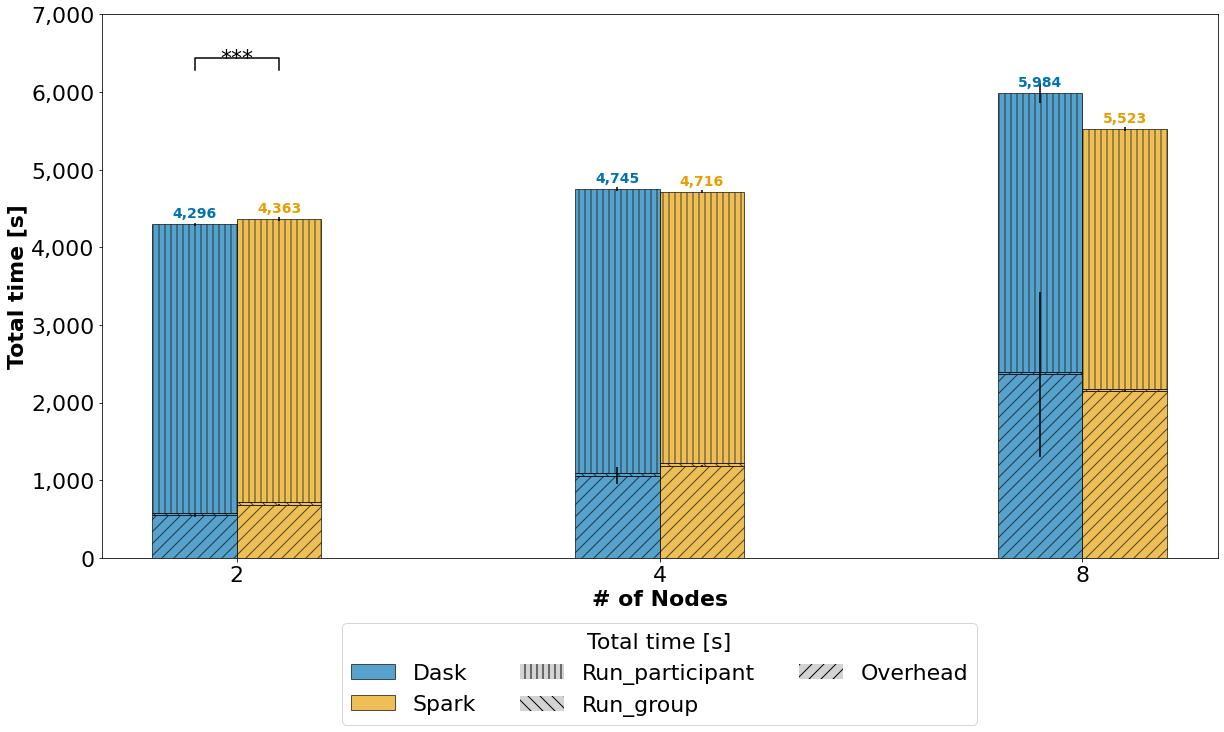
\includegraphics[clip,width=\columnwidth]{figures/stacked_bids.jpg}
	\caption{BIDS App Example: varying nodes}
	\label{fig:bids}
\end{figure}

\section{Discussion}
% TODO

\section{Conclusion}
% TODO

\section*{Acknowledgment}
% TODO


\bibliographystyle{IEEEtran}
\bibliography{IEEEabrv,reference}
\end{document}
